\begin{figure}[p]
\centering
\captionsetup{justification=raggedright,labelsep=none,singlelinecheck=false,labelformat=boldlabel}
\caption[]{\footnotesize \textbf{: Validation RMSE and subsequent out-of-sample RMSE after each annual model selection.} Validation windows contain 90 months and subsequent forecast blocks normally contain 12 months. Neural-network validation uses one fitted network, while out-of-sample forecasts average ten independent refits. Differences may therefore reflect refitting, sample length, and changes in volatility conditions.}
\label{fig:rv-validation_test}
\par\smallskip\textbf{Panel A. Long sample}\par\smallskip
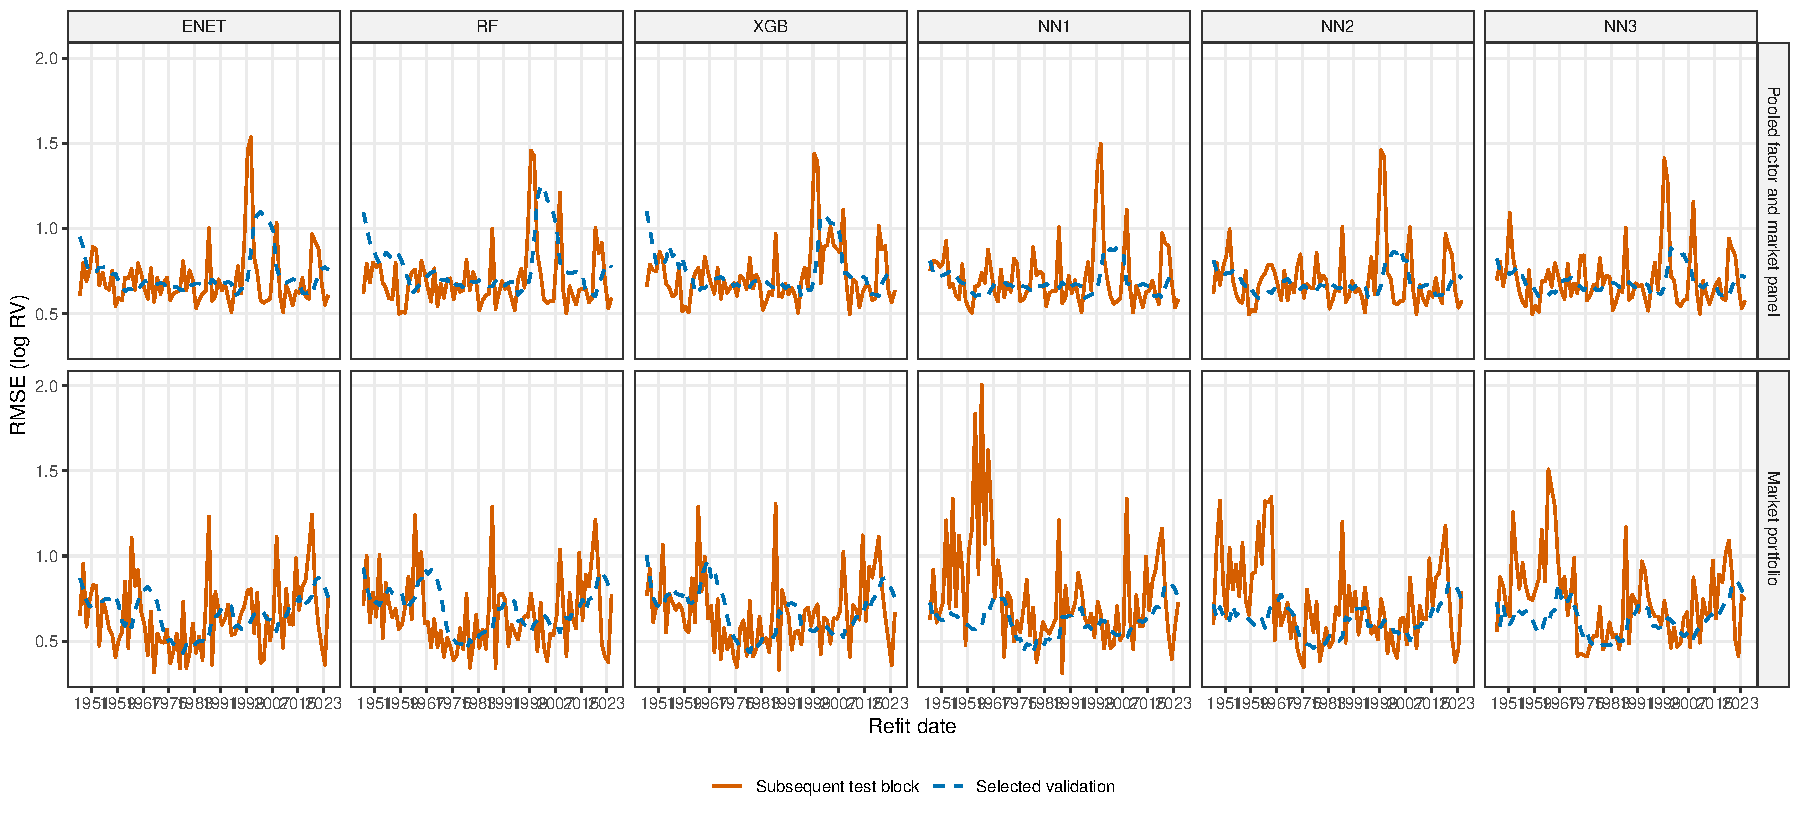
\includegraphics[width=\linewidth,height=0.70\textheight,keepaspectratio]{results_v3/1927/internet_appendix/validation_test.pdf}
\end{figure}
\begin{figure}[p]
\ContinuedFloat
\centering
\captionsetup{justification=raggedright,labelsep=none,singlelinecheck=false,labelformat=boldlabel}
\caption[]{\footnotesize \textbf{: Validation RMSE and subsequent out-of-sample RMSE after each annual model selection.} Validation windows contain 90 months and subsequent forecast blocks normally contain 12 months. Neural-network validation uses one fitted network, while out-of-sample forecasts average ten independent refits. Differences may therefore reflect refitting, sample length, and changes in volatility conditions. Continued.}
\par\smallskip\textbf{Panel B. Short sample}\par\smallskip
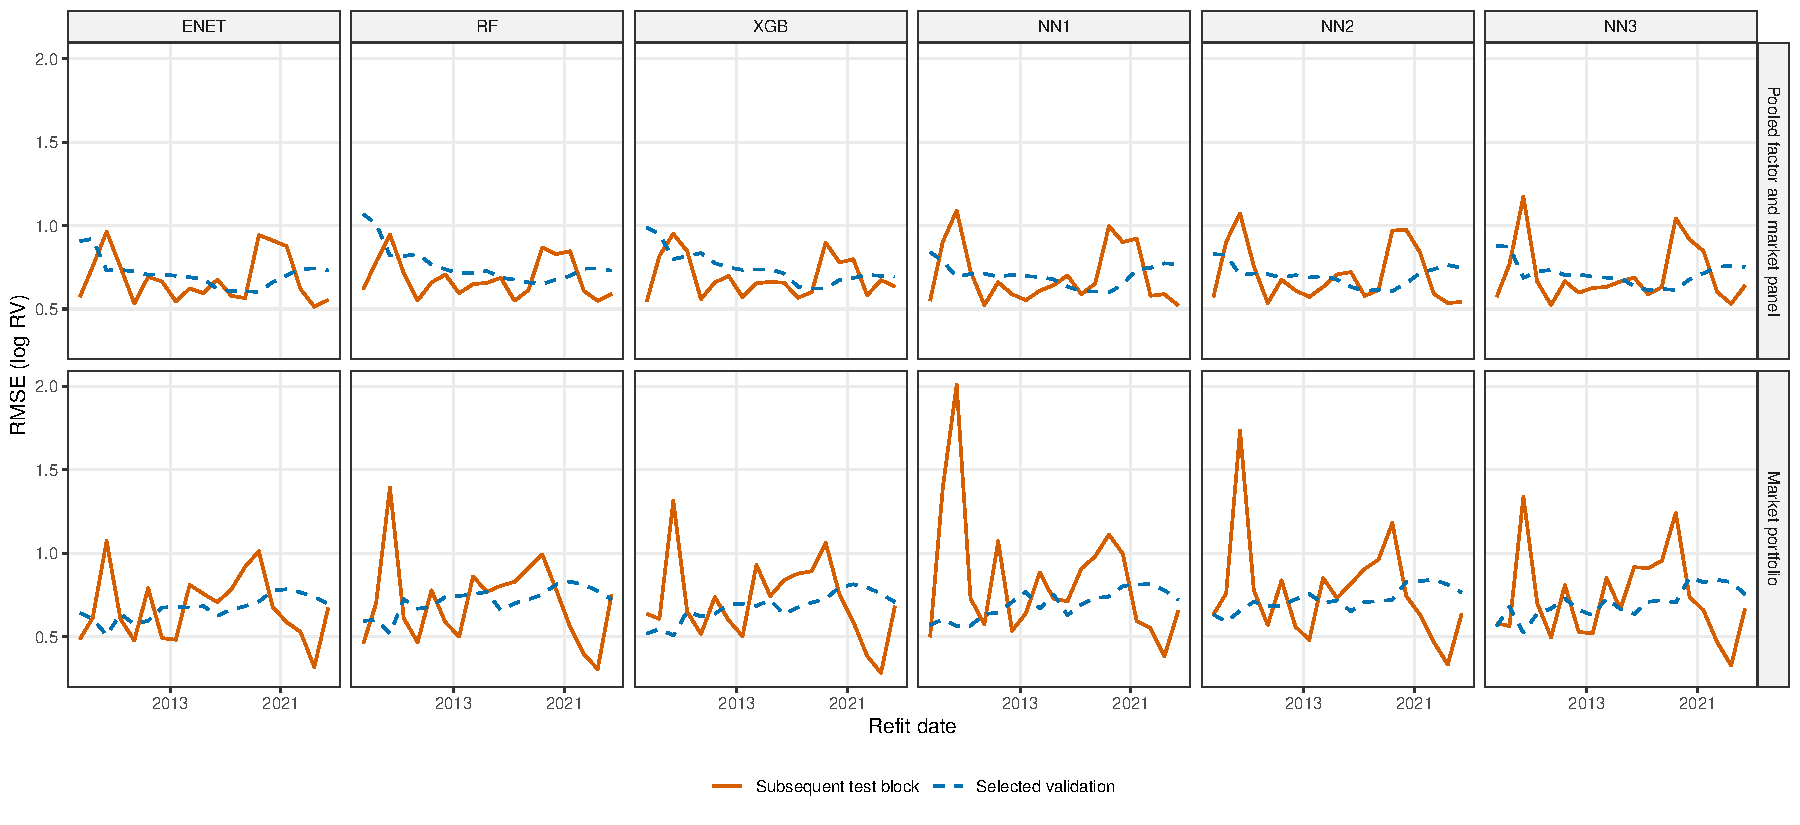
\includegraphics[width=\linewidth,height=0.70\textheight,keepaspectratio]{results_v3/1986/internet_appendix/validation_test.pdf}
\end{figure}
